\documentclass[11pt]{article}
%%%  Topic:   Tikz-Article
%%%	Auother: Daniel Alvarez
%%% Date: 04/30/2019
\usepackage[paper=letterpaper,total={8.0in,9.4in}, top=0.7in, left=.1in]{geometry}

\usepackage{tikz}

\usepackage{float}
\usepackage{verbatim}
\usepackage{textcomp}

\usetikzlibrary{calc}
\usetikzlibrary{decorations, decorations.text,backgrounds}
%COLORS
%reds
\definecolor{cus-red}{RGB}{	254, 82, 88}
\definecolor{cus-red1}{RGB}{241, 14, 22}
\definecolor{cus-red2}{RGB}{251,62,4}
%blues
\definecolor{cus-blue}{RGB}{82, 203, 254}
\definecolor{cus-blue1}{RGB}{14, 173, 241}
\definecolor{cus-blue2}{RGB}{9, 115, 161}
\definecolor{cus-blue3}{RGB}{4,111,251}
%oranges
\definecolor{cus-orange}{RGB}{254, 134, 82}
\definecolor{cus-orange1}{RGB}{254, 144, 4}

\definecolor{cus-sky}{RGB}{85,213,255}
\definecolor{cus-green}{RGB}{29,181,97}
\definecolor{cus-aqua}{RGB}{91, 236, 221}
\definecolor{cus-purp}{RGB}{178, 89, 238}

\definecolor{cus-yellow}{RGB}{254, 191, 82}
\definecolor{cus-green1}{RGB}{148, 238, 89}
\definecolor{cus-violet}{RGB}{148, 238, 89}
\definecolor{branches}{RGB}{147, 98, 1}
\definecolor{cus-tur}{RGB}{9, 161, 156}
\definecolor{cus-white}{RGB}{250,250,250}
\definecolor{cus-black}{RGB}{111,113,114}

%TRIANGLE OBJECTS


\newcommand{\circtri}[1]{
	
	\begin{scope}[xshift=#1 cm]
		\foreach \x in {-8,-7.95,...,7}{
			\foreach \c in { cus-blue,cus-red,cus-orange,cus-yellow,cus-blue1,cus-red1,cus-green,
				cus-aqua,cus-purp,cus-blue2,cus-green1,cus-violet}{
				\draw [thick,rotate=rand*360,xshift=\x*.6 cm,fill=\c,scale=\x*.1] (0 ,0)--(1 ,2)--(2 ,0) -- cycle; 	
			}
		}
	\end{scope}
}
	
\newcommand{\triforce}[5]{
	\begin{scope}[xshift=#1 cm, yscale=#2,yshift=#5 cm]
		\draw [thick,red,fill=#3] (0 ,0)--(1,1.73)--(2 ,0) -- cycle; 
		\draw [thick,rotate around ={60:(0 ,0)},fill=#4] (0 ,0)--(1,1.73)--(2 ,0) -- cycle; 
		\draw [thick,rotate around ={60:(1 ,1.73)},fill=#4] (0 ,0)--(1,1.73)--(2 ,0) -- cycle; 
		\draw [thick,rotate around ={60:(2 ,0)},fill=#4] (0 ,0)--(1,1.73)--(2 ,0) -- cycle;	
\end{scope}
}
\newcommand{\tritile}[1]{
	\begin{scope}[scale=#1]
	\foreach \x in {-10,-6,...,6}{
		\foreach \y in {6,2.5,-1,...,-15}{
			\triforce{\x}{1}{black}{cus-purp}{\y}
		}
	}
	\foreach \x in {-8,-4,...,4}{
		\foreach \y in {-6,-2.5,...,15}{
			
			\triforce{\x}{-1}{black}{cus-orange}{\y}
		}
	}
	\end{scope}
}
\newcommand{\hexagon}[5]{
	\begin{scope}[xshift = #1 cm, yshift = #2 cm,rotate = #5]
		\foreach \c [count=\r from 1] in {#3,#4,#3,#4,#3,#4}{
			\draw [thick,rotate around ={\r*60:(0 ,0)},fill=\c] (0 ,0)--(1,1.73)--(2 ,0) -- cycle; 
		}
\end{scope}
}

\newcommand{\pentagon}[5]{
	\begin{scope}[xshift = #1 cm, yshift = #2 cm, rotate = #5]
		\foreach \c [count=\r from 1] in {#3,#4,#3,#4,#3}{
			\draw [thick,rotate around ={\r*72:(0 ,0)},fill=\c] (0 ,0)--(1,1.73)--(2 ,0) -- cycle; 
		}
\end{scope}}

\newcommand{\qua}[5]{
	\begin{scope}[xshift = #1 cm, yshift = #2 cm, rotate = #5]
		\foreach \c [count=\r from 1] in {#3,#4,#3,#4}{
			\draw [thick,rotate around ={\r*90:(0 ,0)},fill=\c] (0 ,0)--(1,1.73)--(2 ,0) -- cycle; 
		}
\end{scope}
}

\newcommand{\tri}[5]{
	\begin{scope}[xshift = #1 cm, yshift = #2 cm, rotate = #5]
		\foreach \c [count=\r from 1] in {#3,#4,#3}{
			\draw [thick,rotate around ={\r*120:(0 ,0)},fill=\c] (0 ,0)--(1,1.73)--(2 ,0) -- cycle; 
		}
\end{scope}
}

\newcommand{\duo}[5]{
	\begin{scope}[xshift = #1 cm, yshift = #2 cm, rotate = #5]
		\foreach \c [count=\r from 1] in {#3,#4}{
			\draw [thick,rotate around ={\r*180:(0 ,0)},fill=\c] (0 ,0)--(1,1.73)--(2 ,0) -- cycle; 
		}
	\end{scope}
}

%TABLE OBJECTS


\newcommand{\ntwo}{
	
	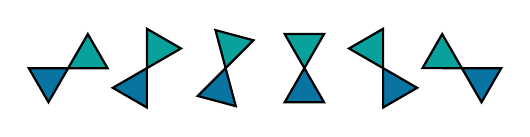
\begin{tikzpicture}
	\begin{scope}[scale = .25]
	\foreach \r [count=\x from 1] in {0,30,45,60,90,120}{
		\duo{\x*4}{0}{cus-blue2}{cus-tur}{\r}
	}
	\end{scope}
	
	\end{tikzpicture}
}


\newcommand{\nthree}{
	
	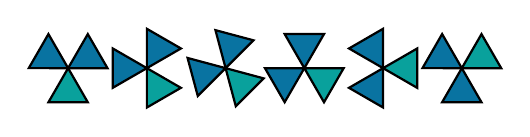
\begin{tikzpicture}
	\begin{scope}[scale = .25]
	\foreach \r [count=\x from 1] in {0,30,45,60,90,120}{
		\tri{\x*4}{0}{cus-blue2}{cus-tur}{\r}
	}
	\end{scope}
	
	\end{tikzpicture}
}

\newcommand{\nfour}{
	
	
\begin{tikzpicture}
	\begin{scope}[scale = .25]
	\foreach \r [count=\x from 1] in {0,30,45,60,90,120}{
		\qua{\x*4}{0}{cus-blue2}{cus-tur}{\r}
	}
	\end{scope}
	
	\end{tikzpicture}
}

\newcommand{\nfive}{
	
	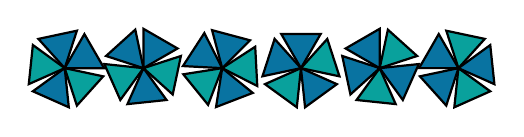
\begin{tikzpicture}
	\begin{scope}[scale = .25]
	\foreach \r [count=\x from 1] in {0,30,45,60,90,120}{
		\pentagon{\x*4}{0}{cus-blue2}{cus-tur}{\r}
	}
	\end{scope}
	
	\end{tikzpicture}
}

\newcommand{\nsix}{
	
	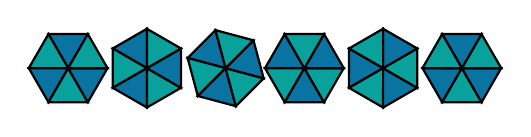
\begin{tikzpicture}
	\begin{scope}[scale = .25]
	\foreach \r [count=\x from 1] in {0,30,45,60,90,120}{
		\hexagon{\x*4}{0}{cus-blue2}{cus-tur}{\r}
	}
	\end{scope}
	
	\end{tikzpicture}
}

%%%%%%%%%%%%%%%%%%%%%%%%%%%%%%%%%%%%%%%%%%%%%%%%%%%%%%%%%%%%%%%%%%%%%%%%%%%%%%%%%%%%
%Pattern Objects
\newcommand{\single}[1]{
	
	\begin{tikzpicture}
	\draw [thick,fill=#1] (0 ,0)--(1,1.73)--(2 ,0) -- cycle;
\end{tikzpicture}
}
\newcommand{\tduo}[7]{
\begin{tikzpicture}[scale = #1,background rectangle/.style={fill=#5}, show background rectangle]
\foreach \x in {#2}{
	\foreach \y in {#3}{
		\duo{\x}{\y}{#6}{#7}{#4}
	}	
}

\end{tikzpicture}
}


\newcommand{\trio}[7]{
	
\begin{tikzpicture}[scale = #1,background rectangle/.style={fill=#5}, show background rectangle]

\foreach \x in {#2}{
	\foreach \y in {#3}{
		\tri{\x}{\y}{#6}{#7}{#4}
	}	
}

\end{tikzpicture}
}
 
\newcommand{\quadr}[7]{
	\begin{tikzpicture}[scale = #1,background rectangle/.style={fill=#5}, show background rectangle]
		\foreach \x in {#2}{
			\foreach \y in {#3}{
				\qua{\x}{\y}{#6}{#7}{#4}
			}	
		}
	\end{tikzpicture}
}
\newcommand{\pent}[7]{
\begin{tikzpicture}[scale = #1,background rectangle/.style={fill=#5}, show background rectangle]
	\foreach \x in {#2}{
		\foreach \y in {#3}{
			\pentagon{\x}{\y}{#6}{#7}{#4}
		}	
	}
\end{tikzpicture}
}
\newcommand{\hex}[7]{
	\begin{tikzpicture}[scale = #1,background rectangle/.style={fill=#5}, show background rectangle]
		\foreach \x in {#2}{
			\foreach \y in {#3}{
				\hexagon{\x}{\y}{#6}{#7}{#4}
			}	
		}
	\end{tikzpicture}
}
\newcommand{\tm}{\texttrademark\xspace}
\newcommand{\degr}[1]{#1$^\circ$}
%###########################################################################################
%###########################################################################################
\begin{document}
	\title{Tikz For More Than Just Math}
	\author{Daniel Alvarez}
	\date{April 03, 2017}
	
	\maketitle
% % % % % % % % % % % % % % % % % % % % % % % % % % % % % % % % % % % % % % % % %
\section{Introduction}
The sole purpose of this article is to demonstrate the use of \emph{Tikz} for projects other than math.
Usually, \emph{Tikz} would be used by professionals in math and the many various fields of science and engineering
to make diagrams. These are usually technical diagrams, for example user manuals, build-it-yourself instructions and  
the diagrams on many exams that we have all experienced at some point. But, unfortunately for those of you who'd like a
demonstration for using tikz for "mathy" projects this is not the article for you. This article will introduce how tikzcan 
be used to make patterns by repeating objects and shapes. In particular my favorite shape the, triangle.I will make the argument that triangles are the only closed shape that we "humans" need to make any other object, 
at least draw any other object.
\\
\paragraph{Squares:}
What do I mean by this ridiculous claim? Well think about it, a square can be 
made up if two right angle triangles, therefore any rectangular object (a square is a rectangle with equal sides) 
can be broken up into triangles of either equal or unequal length sides. For example:\\
%Insert square here
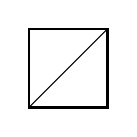
\begin{tikzpicture}[scale = .5]
	\draw (0,0) -- (2,2);
	\draw [thick] (0 ,0) rectangle (2 ,2); 
\end{tikzpicture}
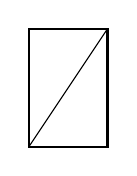
\begin{tikzpicture}[scale = .5]
\draw (0,0) -- (2,3);
\draw [thick] (0 ,0) rectangle (2 ,3); 
\end{tikzpicture}

As you can see, by drawing a diagonal line we can break a square or rectangle into two similar triangles. 

\paragraph{Circles:}
A circle can be approximated by drawing straight lines (edges) to many points (vertices) a circle can be 
made or at least something very near to a perfect circle. Fun fact, any circle you see on a screen is a
not perfect circle. Zoom into any curved surface and you will see that it is not "perfectly" curved. This
is because circle's in math are continuous and have infinite lines that can divide them. Computers understand 1's and
0's which are discreet therefore a computer as we know it cannot understand the concept of continuity. 
Added to that a computer cannot ever calculate numbers to infinity and that includes the infinite decimal numbers between
whole numbers like $1.00000..."$ and whole number infinities. Example:

\begin{center}
	\begin{figure}[H]
		\includegraphics[width=5in]{drW_ngons}
		\caption{Polygon to n}
	\end{figure}
\end{center}

From the figure above it is clear that as more vertices are added the more the polygon "looks" like a circle.
Draw a line from each vertex to the center of the "circle" and it would make a circle approximated by triangles.
In reality, or at least in a computers reality, this is how 2D and 3D objects are made. This concept is heavily
used in the video game and graphics industries.

\subsection{Making a triangle}
Now that you've been convinced that triangles are awesome let me now demonstrate how to make one.
This article will focus on equilateral triangles.
\subsubsection{Equilateral Triangle}
An equilateral Triangle is one with equal length sides that meet at 60 degree angles. Simple 
enough however to draw it in Tikz requires a little knowledge of geometry, particularly one 
Theorem and that is good ole Pythagorus' Theorem.
\begin{displaymath}\label{Pythag}
x^2 + y^2 = h^2
\end{displaymath}
In the case of our triangles x is our base, y is our height and h the hypotenuse. To make
these triangles the I used an x = 2 and h = 2 which implies that the height is $\sqrt{3}$ or
1.72 which is the approximation used in the loops to make multiple triangles.

\begin{tikzpicture}
\draw [very thin , dotted ] (-2,-2) grid (5,5);
%axis
\draw [thick,->] (-2,-2) -- (-2,5);
\node at (-2.2,5){y};
\draw [thick,->] (-2,-2) -- (5,-2);
\node at (5,-2.5){x};
%triangle
\draw [thick] (0 ,0)--(1,1.73)--(2 ,0) -- cycle; 
\draw [thick,|-|,xshift=-.2 cm] (0,0) -- (1,1.73);
\node at (0,1.5){y=2};
\draw [thick, |-|] (-.5,0) -- (-.5,1.73);
\node at (-1.5,1) {h=$\sqrt{3}$};
\draw [thick, |-|] (0,-.5) -- (2,-.5);
\node at (1,-.75) {x=2}; 
\end{tikzpicture}
\newline
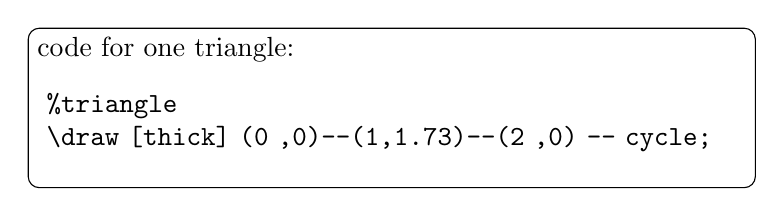
\begin{tikzpicture}
\node [draw , rectangle, rounded corners,text width=9 cm] at (6 ,4) { 
	code for one triangle:
	\begin{verbatim}
	%triangle
	\draw [thick] (0 ,0)--(1,1.73)--(2 ,0) -- cycle; 
	\end{verbatim}
};
\end{tikzpicture}
\section{Adding Triangles}
In this section we'll look at shapes and patterns that can be made by adding together equilateral triangles together at angles. 
\subsection{By Edges}
To have one triangle rest against another perfectly the second triangle will have to be drawn about 60 degrees to any one point. This will add the triangles together by their edges.
For example:
\bigskip
\\
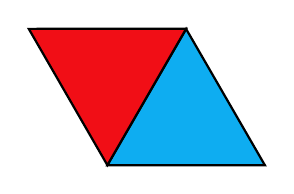
\begin{tikzpicture}
	\draw [thick,fill=cus-blue1] (0 ,0)--(1,1.73)--(2 ,0) -- cycle; 
	\draw [thick,rotate around ={60:(0 ,0)},fill=cus-red1] (0 ,0)--(1,1.73)--(2 ,0) -- cycle; 
\end{tikzpicture}
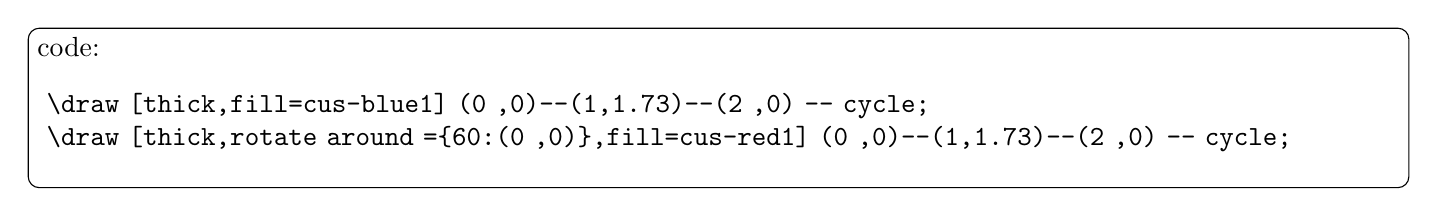
\begin{tikzpicture}
\node [draw , rectangle, rounded corners,text width=17.3 cm] at (6 ,4) { 
	code:
	\begin{verbatim}
	\draw [thick,fill=cus-blue1] (0 ,0)--(1,1.73)--(2 ,0) -- cycle; 
	\draw [thick,rotate around ={60:(0 ,0)},fill=cus-red1] (0 ,0)--(1,1.73)--(2 ,0) -- cycle; 
	\end{verbatim}
};
\end{tikzpicture}
\bigskip
\newline
From the figure above, the red triangle is the same as the one in blue but it is rotated about the point (0,0)  which in this case is the lower left corner of the blue triangle. Rotation in Tikz are done as they are in math
which is that it rotates counterclockwise. Hence the red triangle is to the left of the blue. 
\bigskip
\newline
Adding together these triangles along a vertical axis can produce some nice patterns.
example:\\
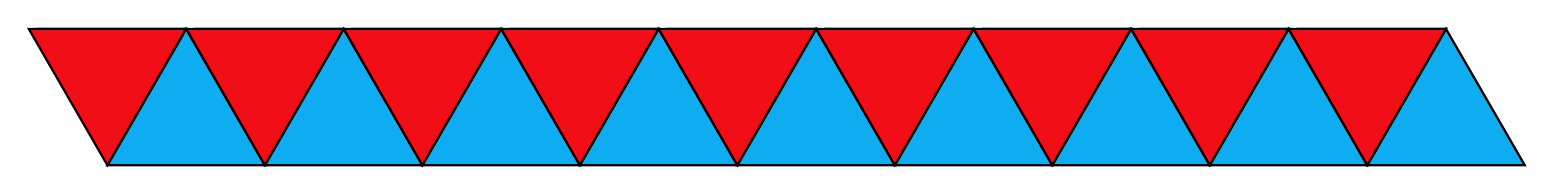
\begin{tikzpicture}
\foreach \x in {2,4,...,18}{
	\begin{scope}[xshift=\x cm]
	\draw [thick,fill=cus-blue1] (0 ,0)--(1,1.73)--(2 ,0) -- cycle; 
	\draw [thick,rotate around ={60:(0 ,0)},fill=cus-red1] (0 ,0)--(1,1.73)--(2 ,0) -- cycle; 
	\end{scope}
}
\end{tikzpicture}
\\
\bigskip
Of course depending on how it's colored various pictures can be drawn. For example coloring a 
light blue with green can convey mountains in your favorite retro NES game (if any of you were alive for that. Fun fact, that was my first console). Example:\\
\bigskip
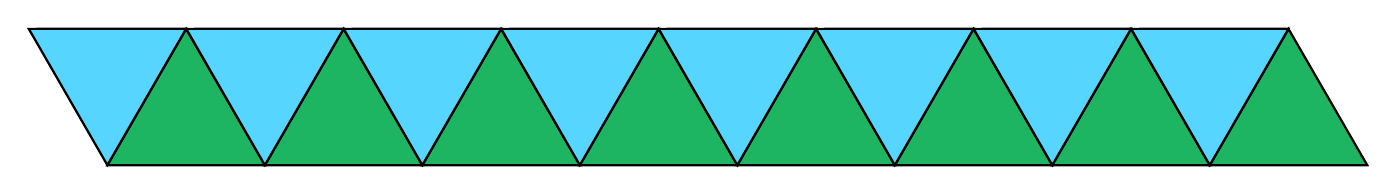
\begin{tikzpicture}
\foreach \x in {2,4,...,16}{
	\begin{scope}[xshift=\x cm]
	\draw [thick,fill=cus-green] (0 ,0)--(1,1.73)--(2 ,0) -- cycle; 
	\draw [thick,rotate around ={60:(0 ,0)},fill=cus-sky] (0 ,0)--(1,1.73)--(2 ,0) -- cycle; 
	\end{scope}
}
\end{tikzpicture}
\\
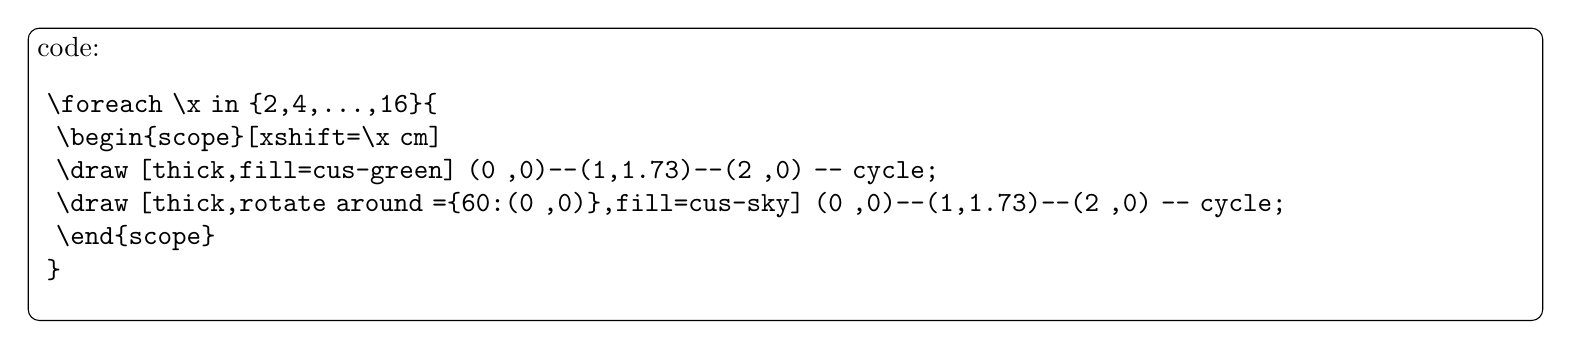
\begin{tikzpicture}[scale = .4]
\node [draw , rectangle, rounded corners,text width=19 cm] at (6 ,4) { 
	code:
	\begin{verbatim}
	\foreach \x in {2,4,...,16}{
		\begin{scope}[xshift=\x cm]
		\draw [thick,fill=cus-green] (0 ,0)--(1,1.73)--(2 ,0) -- cycle; 
		\draw [thick,rotate around ={60:(0 ,0)},fill=cus-sky] (0 ,0)--(1,1.73)--(2 ,0) -- cycle; 
		\end{scope}
	}
	\end{verbatim}
};
\end{tikzpicture}
\bigskip
\\
And of course by adding another we can draw these in both directions:\\
\\
\bigskip
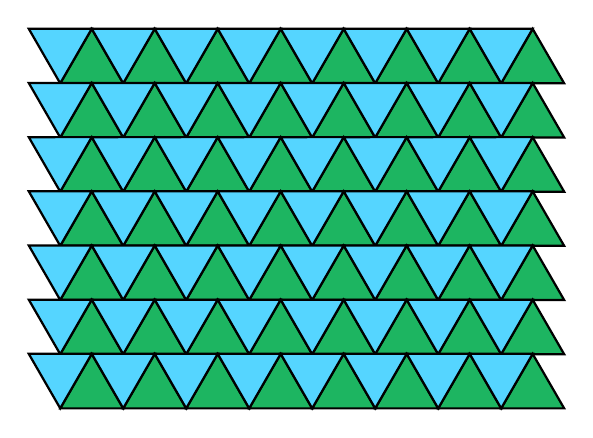
\begin{tikzpicture}[scale = .4]
\foreach \x in {2,4,...,16}{
	\foreach \y in {0,-1.72,...,-10.38}{
		\begin{scope}[xshift=\x cm, yshift=\y cm]
		\draw [thick,fill=cus-green] (0 ,0)--(1,1.73)--(2 ,0) -- cycle; 
		\draw [thick,rotate around ={60:(0 ,0)},fill=cus-sky] (0 ,0)--(1,1.73)--(2 ,0) -- cycle; 
		\end{scope}
}
}
\end{tikzpicture}
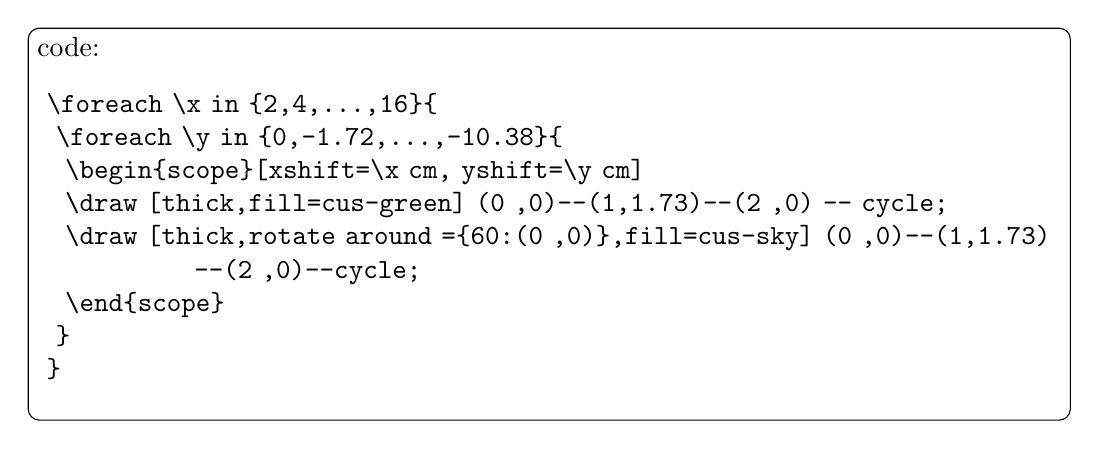
\begin{tikzpicture}[scale = .4]
\node [draw , rectangle, rounded corners,text width=13 cm] at (6 ,4) { 
	code:
	\begin{verbatim}
	\foreach \x in {2,4,...,16}{
		\foreach \y in {0,-1.72,...,-10.38}{
			\begin{scope}[xshift=\x cm, yshift=\y cm]
			\draw [thick,fill=cus-green] (0 ,0)--(1,1.73)--(2 ,0) -- cycle; 
			\draw [thick,rotate around ={60:(0 ,0)},fill=cus-sky] (0 ,0)--(1,1.73)
		 														--(2 ,0)--cycle; 
			\end{scope}
		}
	}
	\end{verbatim}
};
\end{tikzpicture}
\paragraph{NOTE:}
Notice that the inner loop controls the y axis translations of the object and it goes in a range
that is a multiple of 1.72 or $\sqrt{3}$ which in the height of each triangle. Not doing this will
either leave space between the rows of triangles or place them one on top each other. This is of
course up to the artist but for the purpose of this demonstration we require them to touch.

\subsubsection{Triforce}
Anyone who really knows me knows that I am a huge fan of video game
franchise The Legend of Zelda \textsuperscript{TM} . The trademark symbol for this video games is what's referred to as the "Triforce"
which looks like this:
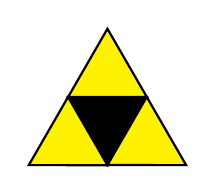
\begin{tikzpicture}[scale = .5]
	\begin{scope}[yscale = -1]
		\draw [thick,fill=black] (0 ,0)--(1,1.73)--(2 ,0) -- cycle; 
		\draw [thick,rotate around ={60:(0 ,0)},fill=yellow] (0 ,0)--(1,1.73)--(2 ,0) -- cycle; 
		\draw [thick,rotate around ={60:(1 ,1.73)},fill=yellow] (0 ,0)--(1,1.73)--(2 ,0) -- cycle; 
		\draw [thick,rotate around ={60:(2 ,0)},fill=yellow] (0 ,0)--(1,1.73)--(2 ,0) -- cycle;
	\end{scope}
\end{tikzpicture}
. Of course as you make many of the same objects it's better to wrap them in \verb|\begin{scope}| environments then making a new command in the preamble and setting 
the possible parameters to whatever you you'd like to manipulate. Therefore the code for this one triforce
is: \\
\\
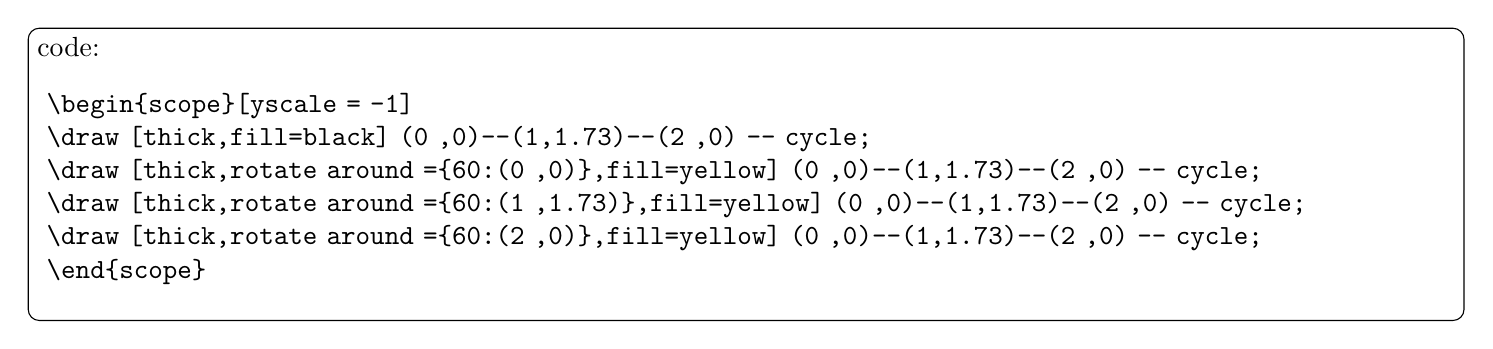
\begin{tikzpicture}[scale = .5]
\node [draw , rectangle, rounded corners,text width=18 cm] at (6 ,4) { 
	code:
	\begin{verbatim}
	\begin{scope}[yscale = -1]
	\draw [thick,fill=black] (0 ,0)--(1,1.73)--(2 ,0) -- cycle; 
	\draw [thick,rotate around ={60:(0 ,0)},fill=yellow] (0 ,0)--(1,1.73)--(2 ,0) -- cycle; 
	\draw [thick,rotate around ={60:(1 ,1.73)},fill=yellow] (0 ,0)--(1,1.73)--(2 ,0) -- cycle; 
	\draw [thick,rotate around ={60:(2 ,0)},fill=yellow] (0 ,0)--(1,1.73)--(2 ,0) -- cycle;
	\end{scope}
	\end{verbatim}
};
\end{tikzpicture}
\\
We then take this code and make a new command called \verb|\triforce{arg1}{arg2}{arg3}{arg4}{arg5}|
like so:\\
\\
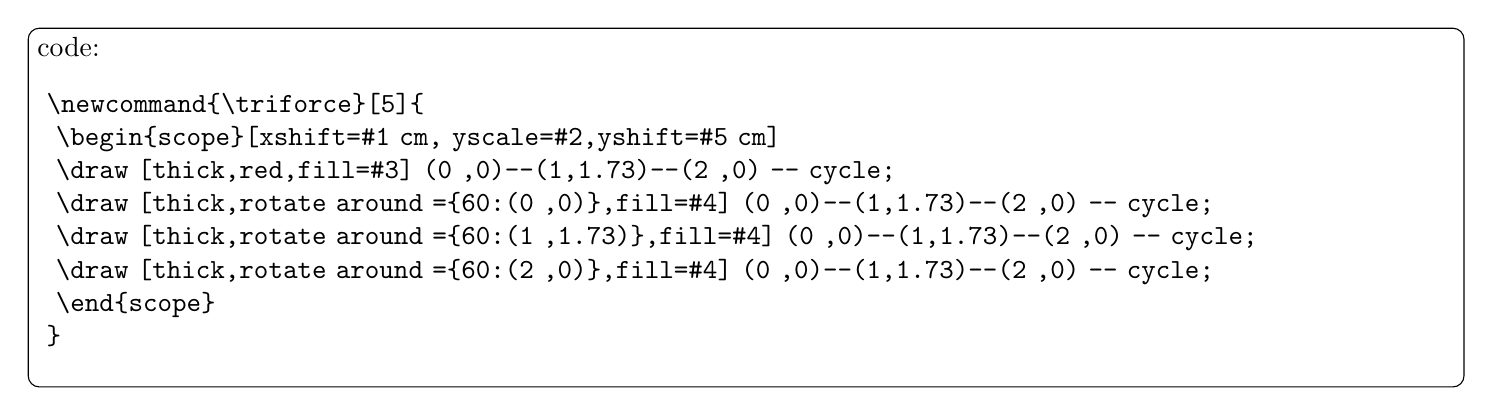
\begin{tikzpicture}[scale = .5]
\node [draw , rectangle, rounded corners,text width=18 cm] at (6 ,4) { 
	code:
	\begin{verbatim}
	\newcommand{\triforce}[5]{
		\begin{scope}[xshift=#1 cm, yscale=#2,yshift=#5 cm]
		\draw [thick,red,fill=#3] (0 ,0)--(1,1.73)--(2 ,0) -- cycle; 
		\draw [thick,rotate around ={60:(0 ,0)},fill=#4] (0 ,0)--(1,1.73)--(2 ,0) -- cycle; 
		\draw [thick,rotate around ={60:(1 ,1.73)},fill=#4] (0 ,0)--(1,1.73)--(2 ,0) -- cycle; 
		\draw [thick,rotate around ={60:(2 ,0)},fill=#4] (0 ,0)--(1,1.73)--(2 ,0) -- cycle;	
		\end{scope}
	}
	\end{verbatim}
};
\end{tikzpicture}
\\
Adding these together in various ways can produce some interesting patterns. I particularly like this
for tiling patterns as shown below:\\
\bigskip
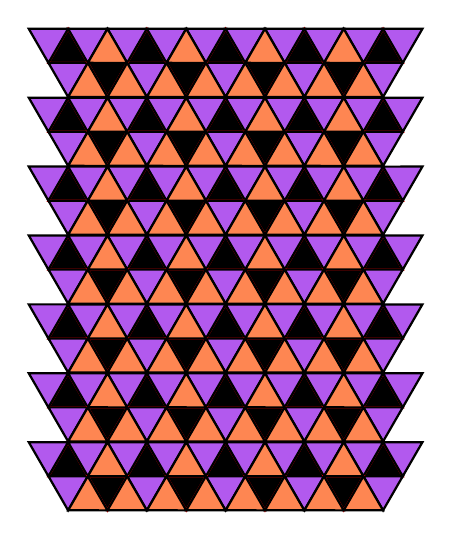
\begin{tikzpicture}[scale = .5]
\tritile{.5}
\end{tikzpicture}
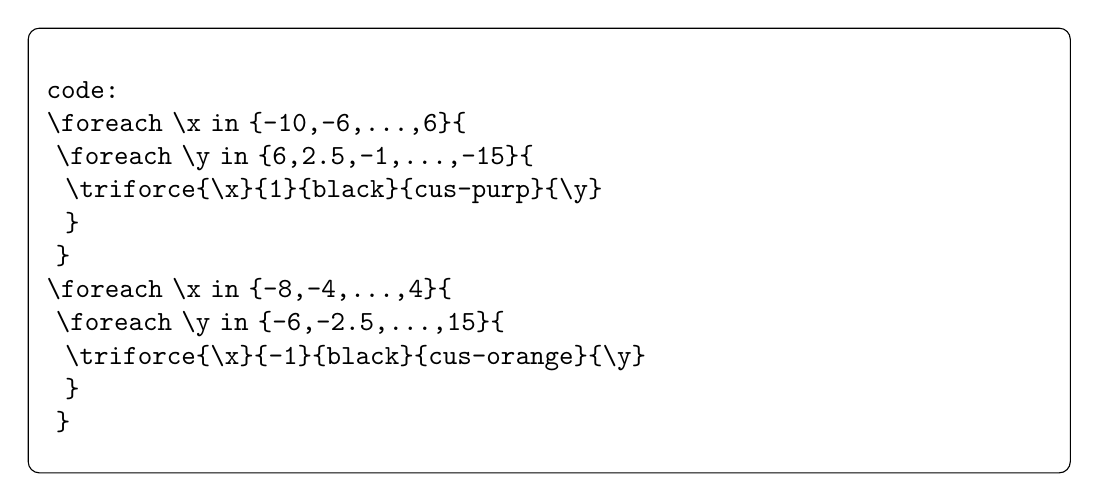
\begin{tikzpicture}[scale = .5]
\node [draw , rectangle, rounded corners,text width=13 cm] at (6 ,4) { 
	
	\begin{verbatim}
	code:
	\foreach \x in {-10,-6,...,6}{
		\foreach \y in {6,2.5,-1,...,-15}{
			\triforce{\x}{1}{black}{cus-purp}{\y}
			}
		}
	\foreach \x in {-8,-4,...,4}{
		\foreach \y in {-6,-2.5,...,15}{
			\triforce{\x}{-1}{black}{cus-orange}{\y}
			}
		}
	\end{verbatim}
};
\end{tikzpicture}
\paragraph{NOTE:}
Notice that the Triforce object is created using \verb|\triforce{\x}{1}{black}{cus-purp}{\y}|
which makes the object with parameters: xshift, yscale, center triangle fill color, outer 
triangle fill color and yshift. It's good practice to be consistent in the order of arguments
but sometimes different objects may require a different order. A neat trick is using xscale and 
yscale to flip objects. Setting xscale = -1 flip horizontally and of course yscale = -1 flips 
vertically.

\subsection{By Vertices}
Now let's take a look at what is possible when triangles are added by there vertices or simply there
corner points. 
\paragraph{Adding at Vertices}

Creating these patterns was done in a very object oriented way. The result
was that it made things easier when wanting to do use the patterns for different
purposes. I may need just one line for a table like table~\ref{patternsTable}
or for an entire as seen in the last section of this article. This process 
involved make an object that is a shape made by n Triangles. I originally made 
a new object for each shape. Starting with n = 2.\\
\bigskip
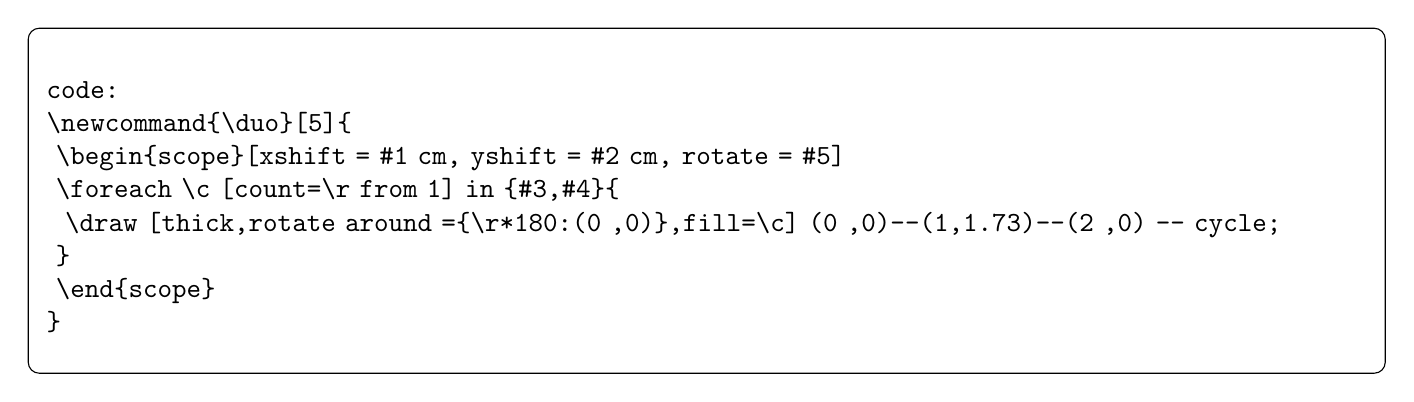
\begin{tikzpicture}[scale = .5]
\node [draw , rectangle, rounded corners,text width=17 cm] at (6 ,4) { 
	
	\begin{verbatim}
	code:
	\newcommand{\duo}[5]{
		\begin{scope}[xshift = #1 cm, yshift = #2 cm, rotate = #5]
		\foreach \c [count=\r from 1] in {#3,#4}{
			\draw [thick,rotate around ={\r*180:(0 ,0)},fill=\c] (0 ,0)--(1,1.73)--(2 ,0) -- cycle; 
		}
		\end{scope}
	}
	\end{verbatim}
};
\end{tikzpicture}
\bigskip
\\
\paragraph{NOTE:}
I wanted to do this using only one for loop for a better run time yet still be able to which sort of 
manipulate color which sort of forced me to make the number of triangles that are created depend
on the colors that are passed in. As is it now arguments \#3 and \#4 are the colors that are passed
in. Then for every triangle that is created the next will be created at the point (0,0) and rotated
by $\frac{360}{n}$ degrees. To add more triangles just add more arguments for the colors i.e 
\verb|\foreach \c [count=\r from 1] in {#3,#4,#3,#4}| for 4 triangles.\\
The code above produces:

\begin{tikzpicture}[scale=.3]
	\duo{0}{0}{cus-blue2}{cus-tur}{60}
\end{tikzpicture}
.\quad
I then created an object called \verb|\ntwo| containing that object to make it easier to make many more
single patterns at different angles as seen in table~\ref{nTriangles} below. I then created an object for
each pattern. Again there is a better way of doing this. 
%Show code in the presentation

\bigskip
\begin{table}[H]
	\centering
	\begin{tabular}{|c| l|}
		\hline
		\textbf{n} & \textbf{angles\{0,30,45,60,90,120\}}\\% chead defined in the preamble
		\hline
		n = 2 &  \ntwo\\
		\hline
		n = 3 &  \nthree\\
		\hline
		n = 4 &  \nfour\\
		\hline
		n = 5 &  \nfive\\
		\hline
		n = 6 &  \nsix\\
		\hline
	\end{tabular}
	\caption{Table of triangle up to n=6}\label{nTriangles}
\end{table}
\bigskip

It can be seen by the table that as more triangles are added it becomes difficult to notice small changes in angle
of rotation does not change by much. In fact had they been all one color it would be difficult so see how they are rotated\\
especially with the close form n=6 pattern.



\section{Combining Patterns}
In this section we'll see how adding together patterns can make more complicated patterns
that once colored in can produce an entirely new visual experience. However, for this to work
at least for the purpose of this article, the shapes must be touching at least in one direction.
To accomplish this yet another object "command" was made to store the shape but this time arguments
were passed in to better manipulate the size, position, rotation and background color of the overall
pattern. For example:\\
\bigskip
\begin{tikzpicture}[scale = .5]
\node [draw , rectangle, rounded corners,text width=19 cm] at (6 ,4) { 
	
	\begin{verbatim}
	code:
	\newcommand{\tduo}[7]{
		\begin{tikzpicture}[scale = #1,background rectangle/.style={fill=#5}, show background rectangle]
		\foreach \x in {#2}{
			\foreach \y in {#3}{
				\duo{\x}{\y}{#6}{#7}{#4}
			}	
		}
		
		\end{tikzpicture}
	}	
	\end{verbatim}
	};
\end{tikzpicture}
	
	\paragraph{NOTE:}
	Notice where the arguments \#2 and \#3 are, this technique proved to be very helpful for changing the 
	range when displaying the pattern for different purposes. For example, I may need just one line for a table like table~\ref{patternsTable}
	below.
	

\begin{table}[H]
	\centering
	\begin{tabular}{|c|l|l|l|}
		\hline
		\textbf{n} & \textbf{1} & \textbf{2} & \textbf{3}\\ %& \textbf{30 degrees} & \textbf{45 degrees}\\% chead defined in the preamble
		\hline
		 Pattern  & \single{cus-tur} & \tduo{.25}{0,4,...,8}{3.46,1.73,...,-5.17}{0}{white}{cus-blue2}{cus-tur} & \trio{.25}{0,4,...,8}{0,-3.46,...,-10.38}{0}{white}{cus-blue2}{cus-tur}\\
		\hline
		\textbf{n} & \textbf{4} & \textbf{5} & \textbf{6}\\ %& \textbf{30 degrees} & \textbf{45 degrees}\\% chead defined in the preamble
		\hline
		Pattern  &  \quadr{.25}{0,3.5,...,7}{0,-3.5,...,-7}{60}{white}{cus-blue2}{cus-tur}	& \pent{.25}{0,4,...,8}{0,-4,...,-8}{0}{white}{cus-blue2}{cus-tur} & \hex{.25}{0,4,...,8}{0,-3.55,...,-10.65}{0}{white}{cus-blue2}{cus-tur}\\
		\hline
		
	\end{tabular}
	\caption{Examples of patterns with n triangles}\label{patternsTable}
\end{table}


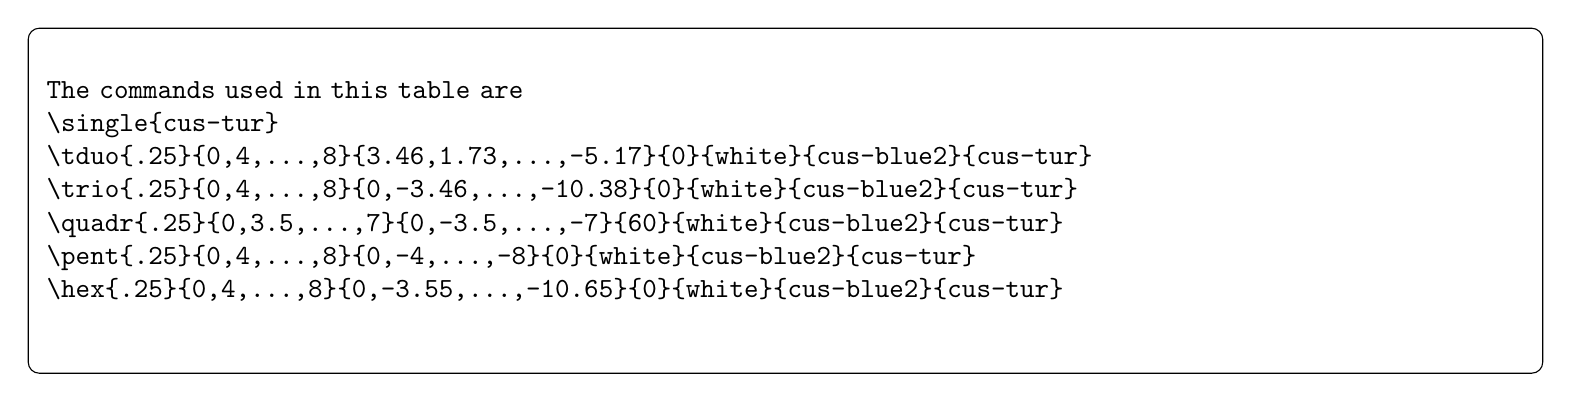
\begin{tikzpicture}
	
\node [draw , rectangle, rounded corners,text width=19 cm] at (6 ,4) { 
	
	\begin{verbatim}
	The commands used in this table are
	\single{cus-tur}
	\tduo{.25}{0,4,...,8}{3.46,1.73,...,-5.17}{0}{white}{cus-blue2}{cus-tur}
	\trio{.25}{0,4,...,8}{0,-3.46,...,-10.38}{0}{white}{cus-blue2}{cus-tur}
	\quadr{.25}{0,3.5,...,7}{0,-3.5,...,-7}{60}{white}{cus-blue2}{cus-tur}
	\pent{.25}{0,4,...,8}{0,-4,...,-8}{0}{white}{cus-blue2}{cus-tur}
	\hex{.25}{0,4,...,8}{0,-3.55,...,-10.65}{0}{white}{cus-blue2}{cus-tur}
		
		\end{verbatim}
	};
\end{tikzpicture}
\\
Notice some of the ranges are in multiples of $\sqrt{3}$. This is where knowing the
dimensions of one singular triangle (other any object) is important. 

\section{Patterns}
Below are some examples of larger patterns, for the intentions of this article I chose patterns
created at angles I thought looked better but please play the angle of rotation:
\subsection{Dual Triangles}
\begin{table}[H]
	\centering
	\begin{tabular}{|c|l|l|}
		\hline
		\textbf{Rotation} & \textbf{\degr{0}} & \textbf{\degr{30}}\\
		\hline
		Pattern  & \tduo{.45}{0,4,...,16}{0,-1.73,...,-10.38}{0}{white}{cus-blue2}{cus-tur} & \tduo{.45}{0,1.73,...,15.48}{0,-4,...,-8}{30}{white}{cus-blue2}{cus-tur}\\
		\hline
	\end{tabular}
	\caption{Dual triangle patterns}\label{dualpattern}
\end{table}




% #########################################
\subsection{3 Triangles}
\begin{table}[H]
	\centering
	\begin{tabular}{|c|l|l|}
		\hline
		\textbf{Rotation} & \textbf{\degr{0}} & \textbf{\degr{30}}\\
		\hline
		Pattern  & \trio{.45}{0,4,...,16}{0,-3.46,...,-17.2}{0}{white}{cus-blue2}{cus-tur} & \trio{.45}{0,3.46,...,17.2}{0,-4,...,-16}{30}{white}{cus-blue2}{cus-tur}\\
		\hline
		\textbf{Rotation} & \textbf{\degr{45}} & \textbf{\degr{60}}\\
		 &\trio{.45}{0,3.46,...,17.2}{0,-3.46,...,-17.2}{45}{white}{cus-blue2}{cus-tur}&\trio{.45}{0,3.46,...,17.2}{0,-3.46,...,-17.2}{60}{white}{cus-blue2}{cus-tur}\\
		\hline
	\end{tabular}
	\caption{Triple triangle patterns}\label{triplepattern}
\end{table}


%#################################################
\section*{4 Triangles}
\subsection*{0 degrees}

\begin{table}[H]
	\centering
	\begin{tabular}{|c|l|l|}
		\hline
		\textbf{Rotation} & \textbf{\degr{0}} & \textbf{\degr{30}}\\
		\hline
		Pattern  & \quadr{.4}{0,4,...,16}{0,-4,...,-16}{0}{white}{cus-blue2}{cus-tur} & \quadr{.4}{0,3.46,...,17.2}{0,-3.46,...,-17.2}{30}{white}{cus-blue2}{cus-tur}\\
		\hline
		\textbf{Rotation} & \textbf{\degr{45}} & \textbf{\degr{60}}\\
		Pattern &\quadr{.4}{1,4.5,...,18.5}{0,-3.5,...,-14}{45}{white}{cus-blue2}{cus-tur} &\quadr{.4}{0,3.46,...,17.2}{0,-3.46,...,-17.2}{60}{white}{cus-blue2}{cus-tur} \\
		\hline
	\end{tabular}
	\caption{Quadruple triangle patterns}\label{quadpattern}
\end{table}



%#############################################################
\section*{5 Triangles}


\begin{table}[H]
\centering
\begin{tabular}{|c|l|l|}
	\hline
	\textbf{n Triangles} & \textbf{Five} & \textbf{Six}\\
	\hline
	Patterns  & \pent{.4}{0,4,...,16}{-4,-8,...,-16}{72}{white}{cus-blue2}{cus-tur} & \hex{.4}{0,4,...,16}{0,-3.46,...,-17.2}{0}{white}{cus-blue2}{cus-tur}\\
	\hline
\end{tabular}
\caption{Five and six triangle patterns}\label{penthexpattern}
\end{table}
As seen in table~\ref{nTriangles} patterns with five and six triangles do not
look mush different when the angle is changed. This is however only true because they
are being drawn with only two colors.
 

\section{Using backgrounds}
Notice that each shape takes in an argument for the background. by doing this patterns may be 
created using the negative spaces of the shape. Make sure to include \verb|\usetikzlibrary{decorations, decorations.text,backgrounds}| to get access to the
background color and type (rectangle,circle,etc).
\subsection{Black and White}
The table below shows my personal favorite patterns when drawn in black and white.
Notice how the negative spaces can give the appearance of a completely different pattern
being drawn. This is especially the case for n = 4 as seen below.\\
\quadr{.4}{0,3.46,...,17.2}{0,-3.46,...,-17.2}{60}{black}{white}{white}
\\
\begin{table}[H]
	\centering
	\begin{tabular}{|c|c|}
		\hline
		\textbf{4 triangles at \degr{60}} & \textbf{4 triangles at \degr{30}}\\
		\hline
		\quadr{.3}{0,3.46,...,17.2}{0,-3.46,...,-17.2}{60}{black}{white}{white}  &  \quadr{.3}{0,3.46,...,17.2}{0,-3.46,...,-17.2}{30}{black}{white}{white}\\
		\hline
		\textbf{3 triangles at \degr{0}} & \textbf{5 triangles at \degr{72}}\\
		\hline
		\trio{.3}{0,4,...,16}{0,-3.46,...,-17.2}{0}{black}{white}{white} &  \pent{.3}{0,4,...,16}{-4,-8,...,-16}{72}{black}{white}{white}\\
	
		\hline
	\end{tabular}
	\caption{Favorite Black and White patterns}\label{bwpatterns}
\end{table}
\newpage
\subsection{Multi-Color}
Here are the same patterns in different colors
\\
\begin{table}[H]
	\centering
	\begin{tabular}{|c|c|}
		\hline
		\textbf{4 triangles at \degr{60}} & \textbf{4 triangles at \degr{30}}\\
		\hline
		\quadr{.3}{0,3.46,...,17.2}{0,-3.46,...,-17.2}{60}{cus-blue3}{cus-red2}{cus-orange1}  &  \quadr{.3}{0,3.46,...,17.2}{0,-3.46,...,-17.2}{30}{cus-blue3}{cus-red2}{cus-orange1}\\
		\hline
		\textbf{3 triangles at \degr{0}} & \textbf{5 triangles at \degr{72}}\\
		\hline
		\trio{.3}{0,4,...,16}{0,-3.46,...,-17.2}{0}{cus-blue3}{cus-red2}{cus-orange1} &  \pent{.3}{0,4,...,16}{-4,-8,...,-16}{72}{cus-blue3}{cus-red2}{cus-orange1}s\\
		
		\hline
	\end{tabular}
	\caption{Multi-Color patterns}\label{colorpatterns}
\end{table}




\pagebreak
\section{Extra:Infinite Triangle}
I love the idea of infinity and I love triangles. So why not mix them?

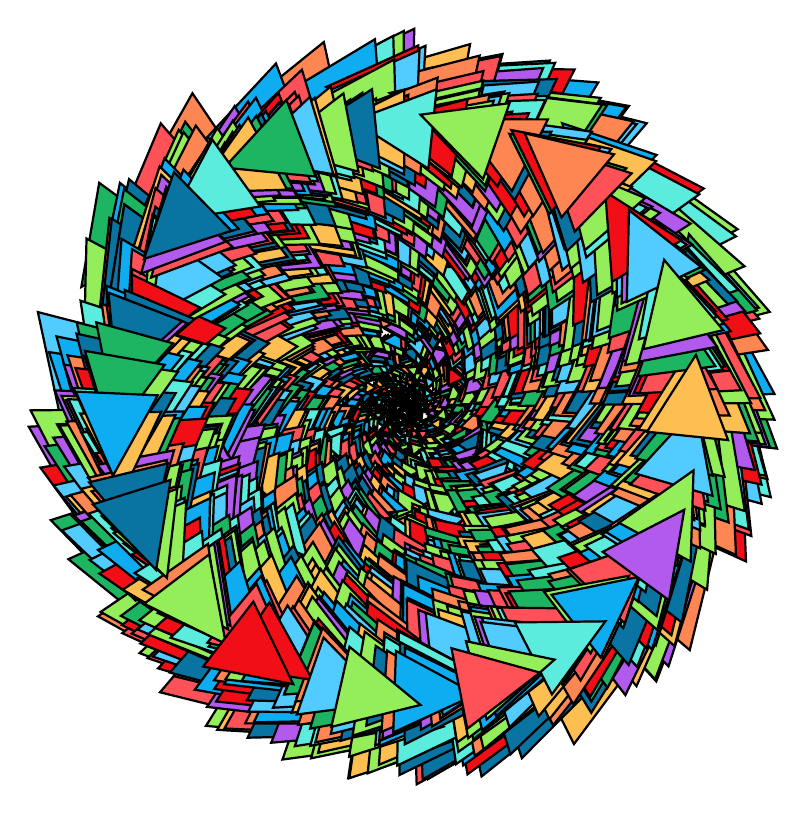
\begin{tikzpicture}[scale=.75]
\circtri{.5}
\end{tikzpicture}
\\
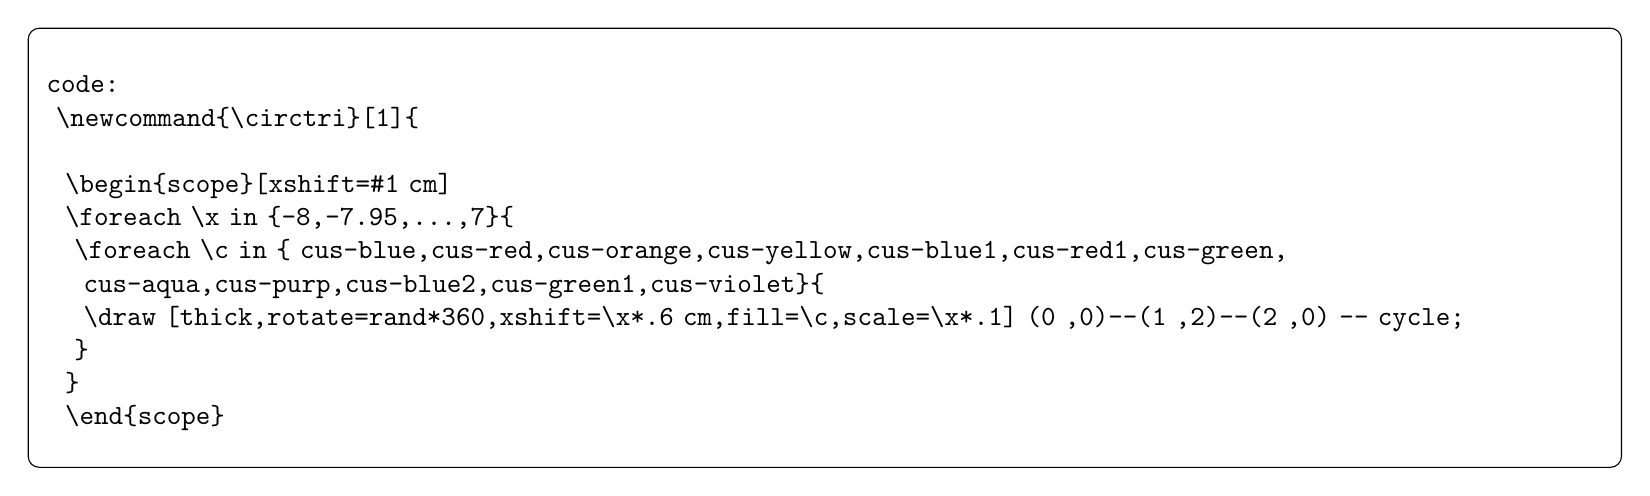
\begin{tikzpicture}[scale = .5]
\node [draw , rectangle, rounded corners,text width=20 cm] at (6 ,4) { 
	\begin{verbatim}
	code:
		\newcommand{\circtri}[1]{
			
			\begin{scope}[xshift=#1 cm]
			\foreach \x in {-8,-7.95,...,7}{
				\foreach \c in { cus-blue,cus-red,cus-orange,cus-yellow,cus-blue1,cus-red1,cus-green,
					cus-aqua,cus-purp,cus-blue2,cus-green1,cus-violet}{
					\draw [thick,rotate=rand*360,xshift=\x*.6 cm,fill=\c,scale=\x*.1] (0 ,0)--(1 ,2)--(2 ,0) -- cycle; 	
				}
			}
			\end{scope}
	\end{verbatim}
};
\end{tikzpicture}
\\
Making this was quite a challenge. I honestly just played around with it's xshift values and using a random
rotation to get get the triangles to move in a circle. Decreasing the scale as triangles are being created collapsed
the picture to the center, that was the key to get the infinity look. Notice that for every xshift value a triangle is
created for every color for every x. Therefore the amount of triangles created per rotation is based on the number of colors,
a similar technique used earlier. Thus there are $(.05 x 15) x 12 = 3,600$ triangles being created.

\end{document}